%\documentclass[12pt,a4paper,oneside]{book}
\documentclass[12pt,a4paper,twoside,twocolumn]{book} % Modelo com duas colunas
%%%%%%%%%%%%%%%%%%%%%%%%%%%%%%%%%%%%%%%%%%%%%%%%%%%%%%%%%%%%%%%%%%%%%%%%%%%%%%%%%%%%%%%%%%%%%%%
\usepackage[brazilian]{babel}
\usepackage[paper=a4paper,text={17.5cm,25.0cm},centering]{geometry}
%\usepackage[text={17cm,24.7cm},centering]{geometry}
%\usepackage[latin1]{inputenc}
\usepackage[utf8x]{inputenc}
\usepackage[T1]{fontenc}
\usepackage{indentfirst}       % indenta os primeiros parágrafos
%------------------------------------------------------------------------------------
%
% \usepackage[english,portuguese]{babel}
% \usepackage[latin9]{inputenc}
% \usepackage{amsmath,amsfonts,amssymb,amsthm}
%
%------------------------------------------------------------------------------------
\usepackage{amsmath,amssymb,amsfonts,amsthm}
\usepackage{bbm}      % Fontes matemáticas para letras gregas em negrito
%\usepackage{bm}        % Fontes matemáticas para letras gregas em negrito
\usepackage{txfonts}   % Gives the lambdabar math symbol
\usepackage{textcomp}  % Símbolos matemáticos p/ modo texto
\usepackage{listings}  % Permite incluir códigos fontes
\usepackage{latexsym}  % Símbolos 
\usepackage{bbold}     % Fontes matemáticas para matrizes
\usepackage{xfrac}     % Fracoes modo texo
%\usepackage{braket}   % introduz bras e kets na mecanica quantica
%
\usepackage{relsize}
%\usepackage{esint}
%\usepackage{multicol}  % Para inserir ambientes com multiplas colunas
\usepackage{multirow}
%\usepackage{supertabular}
%\usepackage[final]{pdfpages}
\usepackage{comment} % Permite inserir comentarios
%\usepackage{chapterbib}  
%\usepackage{makeidx} % Gera indice remissivo
%---------------------------------------------------------------------
\usepackage{graphicx}
\usepackage{thumbpdf}
%\usepackage{color}
\usepackage{rotating}
\usepackage{xcolor}
\usepackage{colortbl}
\usepackage{hyperref}
%---------------------------------------------------------------------
\hypersetup{
   pdfborder={0 0 0},            % Sem caixa em volta da hiperreferência
   pdftoolbar=true,              % Mostra a barra de ferramentas no Acrobat Reader = true ==> sim
   pdfmenubar=true,              % Mostra o menu no Acrobat Reader = true ==> sim
   pdffitwindow=false,           % Ajusta o documento ao tamanho da janela aberta = false==> não
   pdfstartview={FitH},          % Ajusta a largura da página a da janela aberta 
   pdfauthor={Salviano A. Leão}, % Autor do documento
   pdftitle={Modelo de notas de aula},  % Titulo do documento
   pdfsubject={Modelo},          % Assunto do documento
   pdfkeywords={Modelo,notas},  % Palavras chaves do documento
   pdfproducer={LaTeX},    % O produtor do documento
   pdfcreator={pdfLaTeX},  % O programa que criou o documento
   pdfnewwindow=true,      % Abre links em uma nova janela
   colorlinks=true,       % false: links em uma caixa; true: links coloridos
   linkcolor=red,          % Cor dos links internos (mude a cor da caixa com linkbordercolor)
   citecolor=blue,        % Cor dos links das referências bibliográficas
   filecolor=magenta,      % Cor dos links dos arquivos
   urlcolor=cyan           % Cor dos links externos
}
%Note que o último item não tem vírgula.
%--------------------------------------------------------------------
\pdfinfo{%
Title={Mec\^{a}nica Qu\^{a}ntica},
Creator={TeX},
Author={Salviano A. Le\~{a}o},
Subject={Mec\^{a}nica Qu\^{a}ntica},
Keywords={F\'{\i}sica, Mec\^{a}nica Qu\^{a}ntica}
}
%-----------------------------------------------------------------------------------
%\usepackage{breakurl}
\usepackage[aboveskip=4pt,font=small,labelfont=bf,textfont=sl]{caption}
\usepackage[shortlabels]{enumitem}  % Comentei 07/02/2012
%\usepackage{enumerate}               % Descomentei 07/02/2012
%\usepackage{paralist}
%\usepackage{enumerate}
%\usepackage{paralist}
%\usepackage{xypic}
\usepackage[all,knot,arc,import,poly]{xy}
\usepackage{wrapfig}
%\usepackage[geometry]{ifsym}
% \rlap{\VBar}\TriangleUp e \rlap{\TriangleUp}\VBar fornece o simbolo dif-divida
\usepackage{subfig}
%\usepackage{mathpazo}
%\usepackage{floatflt}
%\usepackage{epsf}
%\usepackage{eepic}
%\usepackage{epic}
\usepackage{fancyhdr}
\usepackage{fancybox}
%===============================================================================
\graphicspath{
{Figs/}
{/home/salviano/Cursos/Figs_Logotipos/}
{/home/salviano/Cursos/Figs_Ensino/QM/}
{/home/salviano/Cursos/Figs_Ensino/Mecanica/}
{/home/salviano/Cursos/Figs_Ensino/Fisica_Moderna/}
{/home/salviano/Cursos/Figs_Ensino/Optica/}
{/home/salviano/Cursos/Figs/}
{/home/salviano/Cursos/Figs/eps/}
{/home/salviano/Cursos/Figs_Ensino/Math/}
{/home/salviano/Cursos/Figs_Ensino/Computacao/}
}
%-----------------------------------------------------------------------
\DeclareGraphicsExtensions{.png,.jpg,.pdf,.eps}
%\DeclareGraphicsRule{.jpg}{eps}{.bb}{`jpeg2ps -h -r 100 #1}
\DeclareGraphicsRule{.png}{eps}{.bb}{`convert #1 eps:- } % Conversão on the fly
\DeclareGraphicsRule{.jpg}{eps}{.bb}{`convert #1 eps:- } % Conversão on the fly
%\DeclareGraphicsRule{.eps}{pdf}{.bb}{`epstopdf #1}       % Conversão on the fly
%-----------------------------------------------------------------------
\def\SAL{\bfseries\small \color{red} Prof. Salviano A. Leão}
%-----------------------------------------------------------------------------------
% Macro do Lyx
\DeclareRobustCommand{\lyxmathsym}[1]{\ifmmode\begingroup\def\b@ld{bold}
  \def\rmorbf##1{\ifx\math@version\b@ld\textbf{##1}\else\textrm{##1}\fi}
  \mathchoice{\hbox{\rmorbf{#1}}}{\hbox{\rmorbf{#1}}}
  {\hbox{\smaller[2]\rmorbf{#1}}}{\hbox{\smaller[3]\rmorbf{#1}}}
  \endgroup\else#1\fi}
%===================================================================================
%=========================================================
\newtheorem{theorem}{Teorema}
\newtheorem{acknowledgement}[theorem]{Agradecimentos}
\newtheorem{algorithm}[theorem]{Algoritmo}
\newtheorem{axiom}[theorem]{Axioma}
\newtheorem{case}[theorem]{Caso}
\newtheorem{claim}[theorem]{Declara\c{c}\~{a}o}
\newtheorem{conclusion}[theorem]{Conclu\c{c}\~{a}o}
\newtheorem{condition}[theorem]{Condi\c{c}\~{a}o}
\newtheorem{conjecture}[theorem]{Conjectura}
\newtheorem{corollary}[theorem]{Corol\'{a}rio}
\newtheorem{criterion}[theorem]{Crit\'{\i}rio}
\newtheorem{definition}[theorem]{Defini\c{c}ão}
\newtheorem{postulado}{Postulado}
\newtheorem{example}{Exemplo}
\newtheorem{exercise}{Exerc\'{\i}cio}
\newtheorem{lemma}[theorem]{Lema}
\newtheorem{notation}[theorem]{Nota\c{c}\~{a}o}
\newtheorem{problem}{Problema}
\newtheorem{proposition}[theorem]{Proposi\c{c}\~{a}o}
\newtheorem{remark}[theorem]{Nota}
\newtheorem{solution}{Solu\c{c}\~{a}o}
\newtheorem{summary}[theorem]{Sum\'{a}rio}
%
%\newtheorem{questao}{Quest\~{a}o}
\newtheorem{definicao}{DEFINI\c{C}\~{A}O}
%\newtheorem{definicao}{Defini\c{c}\~ao}
\newtheorem{demonstracao}{Demonstra\c{c}\~{a}o}
\newtheorem{teorema}{Teorema}
\newtheorem{prova}{Prova}
\newtheorem{exemplo}{Exemplo}
\newtheorem{solucao}{Solu\c{c}\~{a}o}
\newtheorem{obs}{Nota}
%\newenvironment{proof}[1][Prova]{\textbf{#1.} }{\ \rule{0.5em}{0.5em}}
%=========================================================
\definecolor{azul_escuro}{rgb}{0.12,0.26, 0.36}
\definecolor{azul}{rgb}{0.21,0.55, 0.0}
\definecolor{Azul}{rgb}{0.21,0.85,0.85}
\definecolor{gold}{rgb}{0.85,.66, 0}
\definecolor{laranja}{rgb}{0.95,.65, 0.20}
\definecolor{Amarelo}{rgb}{0.99,0.99, 0.66}
\definecolor{amarelo}{rgb}{0.95,.95, 0.55}
\definecolor{amarelo1}{rgb}{1,0.97, 0.20}
\definecolor{amarelo2}{rgb}{0.85,0.55, 0.0}
\definecolor{amarelo3}{rgb}{1.0,1.0, 0.80}
\definecolor{verde}{rgb}{0.57,0.94, 0.80}
\definecolor{Cinza50}{gray}{0.50}
\definecolor{Cinza10}{gray}{0.10}
\definecolor{Cinza}{gray}{0.80}
\definecolor{cinza}{rgb}{0.9,0.9,0.9}
%=========================================================
%Definições de tabelas
%-----------------------------------------------------------
\newlength{\LC}
\setlength{\LC}{7.0cm}
\newcolumntype{A}{>{\columncolor[gray]{0.96}\raggedright\color{blue}}l}
\newcolumntype{B}{>{\columncolor[gray]{0.96}\raggedright\color{blue}}r}
\newcolumntype{F}{>{\columncolor[gray]{0.95}\raggedright}m{\LC}}
\newcolumntype{G}{>{\columncolor[gray]{0.9}\raggedright}m{1.70cm}}
\newcolumntype{K}{>{\columncolor[gray]{0.8}\raggedright}c}
\newcolumntype{H}{>{\columncolor{yellow}\raggedright}c}
%=========================================================
\def\ff#1{\hbox{\rm #1}\,}
%\def\fff#1{\hbox{\rm #1}\,}
\def\abs{\ff{abs}}
%\def\acos{\ff{acos}}
%\def\acosh{\ff{acosh}}
%\def\asin{\ff{asin}}
%\def\asinh{\ff{asinh}}
%\def\asin{\ff{atan}}
%\def\atanh{\ff{atanh}}
%\def\sin{\ff{sin}}
%\def\sen{\ff{sen}}
%\def\asen{\ff{asen}}
\def\asinh{\ff{asinh}}
%\def\asen{\ff{atg}}
\def\atanh{\ff{atanh}}
%\def\sen{\ff{sen}}
%\def\cos{\ff{cos}}
%\def\tan{\ff{tan}}
\def\sinh{\ff{sinh}}
\def\cosh{\ff{cosh}}
\def\tanh{\ff{tanh}}
\def\log{\fff{log}}
\def\tg{\ff{tg}}
\def\senh{\ff{senh}}
\def\tgh{\ff{tgh}}
\def\arctg{\ff{arc}\; \ff{tg}}
%=========================================================
\def\lambdabar{\protect\@lambdabar}
\def\@lambdabar{\relax
\bgroup
\def\@tempa{\hbox{\raise.73\ht0
\hbox to0pt{\kern.25\wd0\vrule width.5\wd0
height.1pt depth.1pt\hss}\box0}}\mathchoice{\setbox0\hbox{$\displaystyle\lambda$}\@tempa}{\setbox0\hbox{$\textstyle\lambda$}\@tempa}{\setbox0\hbox{$\scriptstyle\lambda$}\@tempa}{\setbox0\hbox{$\scriptscriptstyle\lambda$}\@tempa}\egroup
}
%=========================================================

% Possiveis Campos
\newcommand{\RR}{\mathbbm{R}}
\newcommand{\CC}{\mathbbm{C}}
\newcommand{\FF}{\mathbbm{F}}
\newcommand{\NN}{\mathbbm{N}}
\newcommand{\ZZ}{\mathbbm{Z}}
\newcommand{\PP}{\mathbbm{P}}
\newcommand{\QQ}{\mathbbm{Q}}
\newcommand{\UU}{\mathbbm{U}}
\newcommand{\EE}{\mathbbm{E}}

% Possiveis Espacos
\def\FF{\mathbb{F}}


%\def\limfunc#1{\mathop{\rm #1}}
\def\func#1{\mathop{\rm #1}\nolimits}
%\def\ve#1{\hat{\mathbf{e}}_{ #1}}
%\def\unit#1{\mathop{\rm #1}\nolimits}
\def\sen{\mathop{\rm sen}\nolimits}
\def\senh{\mathop{\rm senh}\nolimits}
\def\tg{\mathop{\rm tg}\nolimits}
\def\vu#1{\hat{\mathbf{e}}_{#1}}
\def\dvu#1{\dot{\hat{\mathbf{e}}}_{#1}}

\def\Sop#1{\text{\textlbrackdbl} #1 \text{\textrbrackdbl}}
\def\Ort#1#2{R_{\hat{\mathbf{ #1 }}}( #2 )}
\def\Ortd#1#2{R^{\dagger}_{\hat{\mathbf{ #1 }}}( #2 )}
\def\Rt#1#2{\mathcal{R}_{\hat{\mathbf{ #1 }}}( #2 )}
\def\PB{\mathcal{P}}
\def\EF{\mathcal{F}}
\def\EV{\mathbb{V}}
\def\ER{\mathcal{E}_{\mathbf{r}}}
\def\ES{\mathcal{E}_{\mathbf{s}}}
\def\EE{\mathcal{E}}
\def\ket#1{{| #1 \rangle}}
\def\bra#1{{\langle #1 |}}
\def\proj#1#2{  \vert #1 \rangle \langle #2 \vert }
\def\PI#1#2{{\langle #1 | #2 \rangle}}
%\def\PI#1#2{\Braket{ #1 | #2 }}
\def\pbpi#1#2{{\left\vert \langle #1 \vert #2 \rangle \right\vert^2}}
\def\EM#1#2#3{{\left\langle #1 \right| #2 \left| #3 \right\rangle}}
%\def\EM#1#2#3{\Braket{ #1 | #2 | #3 }}
\def\VM#1{\langle #1 \rangle}
\def\TP#1{{\wp}_{if}( #1 )}
\def\dtp#1{\delta {\wp} ( #1 )}
\def\OverBrace#1#2{ \overset{ #1 }{ \overbrace{ #2 } } }
\def\Norm#1{\vert #1 \vert }
\def\Norma#1{\lVert #1 \rVert }
\def\Compl#1{{| #1 \rangle} \langle #1 |}
%\def\RP{\mathbf{R}{\limits}_{\perp}}

\def\Tr#1{\operatorname{tr}(#1)}


\def\mtext#1{{\qquad  \text{#1} \qquad}}
\def\implica{{\qquad  \Longrightarrow \qquad}}

%=========================================================
\newcommand{\eqdef}{\ensuremath{\mathrel{\stackrel{\mathrm{def}}{=}}}}
\newcommand{\eqincert}{\ensuremath{\mathrel{\stackrel{\mathrm{?}}{=}}}}

%===================================================================================
% Redefine os labels dos item
%
% \def\labelitemi{\(\Rightarrow\)}
% \def\labelitemii{\(\rhd\)}
% \def\labelitemiii{\(\bullet\)}
% \def\labelitemiv{\(\star\)}
%=========================================================

%-----------------------------------------------------------------------------------

% \newcommand{\Nota}[1]{%
% \begin{center}
%    \colorbox{amarelo}{\parbox{0.8\linewidth}{ #1}}
% \end{center}}%

% \newcommand{\Nota}[1]{%
% \begin{center}
%    \colorbox{amarelo}{\parbox{0.8\linewidth}{ #1}}
% \end{center}}%
%
% \newcommand{\nota}[1]{%
% \begin{center}
%    \colorbox{amarelo}{\parbox{1.0\linewidth}{ #1}}
% \end{center}}%

\newcommand{\Nota}[1]{%
\begin{center}
   %\colorbox{Azul}{\parbox{0.8\linewidth}{\textbf{NOTA:~} #1}}
   %\shadowbox{\parbox{0.8\linewidth}{\textbf{NOTA:~} #1}}
   \shadowbox{\parbox{0.8\linewidth}{ #1}}
\end{center}}%

\newcommand{\nota}[1]{%
\begin{center}
   %\colorbox{amarelo}{\parbox{1.0\linewidth}{ #1}}
   \shadowbox{\parbox{1.0\linewidth}{ #1}}
\end{center}}%

\newcounter{tarefa}
\newcommand{\Tarefa}[1]{%
\stepcounter{tarefa}
\begin{center}
   \colorbox{Amarelo}{\parbox{0.8\linewidth}{\textbf{TAREFA \arabic{tarefa}:~} #1}}
\end{center}}%

\newcommand{\Mais}[1]{%
\begin{center}
   \colorbox{verde}{\parbox{0.8\linewidth}{\textcolor{red}{\textbf{Para Saber Mais:}}~ #1}}
\end{center}}%

%\newcounter{nota}

%-----------------------------------------------------------------------------------
% \lstnewenvironment{code}{%
% \lstset{frame=single,escapeinside=~~,
% backgroundcolor=\color{black!50},
% basicstyle=\footnotesize\ttfamily}
% }{}

\lstset{%
        inputencoding=utf8,
        extendedchars=true,
        literate=%
        {é}{{\'{e}}}1
        {è}{{\`{e}}}1
        {ê}{{\^{e}}}1
        {ë}{{\¨{e}}}1
        {É}{{\'{E}}}1
        {Ê}{{\^{E}}}1
        {û}{{\^{u}}}1
        {ù}{{\`{u}}}1
        {â}{{\^{a}}}1
        {à}{{\`{a}}}1
        {á}{{\'{a}}}1
        {ã}{{\~{a}}}1
        {Á}{{\'{A}}}1
        {Â}{{\^{A}}}1
        {Ã}{{\~{A}}}1
        {ç}{{\c{c}}}1
        {Ç}{{\c{C}}}1
        {õ}{{\~{o}}}1
        {ó}{{\'{o}}}1
        {ô}{{\^{o}}}1
        {Õ}{{\~{O}}}1
        {Ó}{{\'{O}}}1
        {Ô}{{\^{O}}}1
        {î}{{\^{i}}}1
        {Î}{{\^{I}}}1
        {í}{{\'{i}}}1
        {Í}{{\~{Í}}}1
}

\lstnewenvironment{maxima}{%
\lstset{
frame=single,
escapeinside=~~,
%language=maxima,
inputencoding=utf8x,
stringstyle=\footnotesize\ttfamily
showstringspaces=false,
backgroundcolor=\color{amarelo},
keywordstyle=\color{black}\bfseries,
basicstyle=\footnotesize\ttfamily}
}{}

\lstnewenvironment{code}{%
\lstset{%
        backgroundcolor=\color{Cinza},
        tabsize=3,
        escapeinside=~~,
        rulecolor=,
        language=bash,
        %basicstyle=\scriptsize,
        basicstyle=\footnotesize\ttfamily,
        upquote=true,       % needs package textcomp
        aboveskip={1.5\baselineskip},
        columns=fixed,
        showstringspaces=false,
        extendedchars=true,
        breaklines=true,
        prebreak = \raisebox{0ex}[0ex][0ex]{\ensuremath{\hookleftarrow}},
        frame=single,
        showtabs=false,
        showspaces=false,
        showstringspaces=false,
        identifierstyle=\ttfamily,
        keywordstyle=\color[rgb]{0,0,1}\bfseries,
        %keywordstyle=\color{black}\bfseries,
        commentstyle=\color[rgb]{0.133,0.545,0.133},
        %stringstyle=\color[rgb]{0.627,0.126,0.941},
        stringstyle=\footnotesize\ttfamily}
}{}



%-----------------------------------------------------------------------------------
%\input{Sal_Def}
%-----------------------------------------------------------------------------------
%\pagestyle{fancy}
%\setlength{\headrulewidth}{0.6pt}
% \renewcommand{\headrulewidth}{0.6pt}
% \addtolength{\headwidth}{\marginparsep}
% \lhead[\fancyplain{}{\bfseries Prof. Salviano A. Leão}]%
%       {\fancyplain{}{\bfseries Prof. Salviano A. Leão}}
% \rhead[\fancyplain{}{\bfseries\leftmark}]%
%       {\fancyplain{}{\bfseries\thepage}}
% \cfoot{}


\pagestyle{fancy}
%\fancyhfoffset[LE]{1.40cm}
%\fancyhfoffset[RO]{1.40cm}
\renewcommand{\headrulewidth}{0.8pt}
\renewcommand{\footrulewidth}{0.4pt}
\addtolength{\headwidth}{\marginparsep}
\fancyhead{} % clear all header fields
\fancyfoot{} % clear all footer fields
\fancyhead[LE,LO]{\slshape \nouppercase{\rightmark}}
%\fancyhead[RE,RO]{\slshape Questão \arabic{thequestao}}
\fancyfoot[LE,LO]{\SAL}
%\fancyfoot[CE,CO]{\nouppercase{\rightmark}}
\fancyfoot[RE,RO]{\thepage}
%-------------------------------------------------------------------------------------
%\setlength{\textwidth}{17.0cm}
%\setlength{\textheight}{24.5cm}
%\setlength{\parindent}{1.0cm}
%\setlength{\baselineskip}{0.8cm}
%\voffset=-2.0cm
%\hoffset=-1.0cm
\renewcommand{\baselinestretch}{1.25}
\renewcommand{\textfraction}{0.03}
\renewcommand{\topfraction}{0.97}
\renewcommand{\bottomfraction}{0.97}
\pagestyle{plain}
%-------------------------------------------------------------------------------------


%\makeindex  % Para gerar o indice remissivo

\begin{document}

\begin{titlepage}
\thispagestyle{empty}
\vspace*{-1.0cm}

\begin{center}
\includegraphics[width=0.90\linewidth]{Cab_IF_PB_01.eps}
\end{center}

\vspace*{3.0cm}
\begin{center}
\textbf{\LARGE NOTAS DE AULAS  }
\end{center}
\vspace{5.0cm}

\begin{center}
\textbf{\Huge MECÂNICA QUÂNTICA}
\end{center}
\vspace{\fill}

\begin{center}
{\LARGE \textbf{Prof.:} Dr. Salviano A. Le{\~{a}}o}
\vspace*{1.0cm}

{\Large \textbf{Goi\^{a}nia \today} }
\end{center}
\end{titlepage}

\pagestyle{empty}

\pagebreak
\newpage

\hfill
\newpage

\pagenumbering{roman}
\pagestyle{fancy}
%\pagestyle{plain}
\setcounter{page}{1}

\tableofcontents

\newpage

\pagenumbering{arabic}
\setcounter{page}{1}

\chapter{Introdução}

\section{Elementos de um Circuito}

O livro de eletromagnetismo ideal é o do Griffiths 
\cite{GriffithsEletro}, o qual porém o 
do \cite[ver pag.10]{Adams1992,Niguem2013}.

Para analisarmos\cite{Campos2001,Heath1997,Dahlquist1974} um circuito 
precisamos conhecer os elementos que compõem o
mesmo. Vamos fazer um teste para citar \cite{Tort2001,Adams1992}.

Será feita uma simulação numérica\cite{Conte1980} dos resultados, e
para tal \ldots

\begin{equation}\label{eq:Sch} 
   i \hbar \dfrac{\partial \psi}{\partial t} = H \psi
\end{equation} 

\begin{postulado}
   Enuncia-se o postulado 1
\end{postulado}


\subsection{Resistor}

Um resistor (ôhmico, ou seja, aquele que obedece a lei de Ohm, $V=RI$)
é um elemento de circuito, representado pelo símbolo da figura 
\ref{fig:Resistor}. A lei de Ohm nos diz que: Quando por um resistor R passar
uma corrente I, haverá uma queda de potencial (no sentido da corrente:
$V=V_{1}-V_{2}$; $V_{1}>V_{2}$), através dos seus extremos 1 e 2, dada
por:
\begin{equation*}
V=RI
\end{equation*}

\begin{figure}[!h]
\begin{center}
\includegraphics[width=0.70\linewidth]{Resistor_02.eps}
\end{center}
\caption{Resistor}
\label{fig:Resistor}
\end{figure}


Num resistor, há uma conversão de energia elétrica em energia
térmica, dada pelo efeito Joule. A potência dissipada pelo resistor
devido ao efeito Joule é dada por\cite{RLandau97,DeVries93}:
\begin{equation*}
P=RI^{2}=VI
\end{equation*}

\begin{equation}
M =
\begin{pmatrix}
1/a & x & x \\
-\cos\gamma/(a\sin\chi) & 2 & x \\
x & x & 3
\end{pmatrix}
\end{equation}

Na superfície da figura

\begin{figure}[!h]
\begin{center}
\includegraphics[width=0.70\linewidth,angle=-90]{Superficie.eps}
\end{center}
\caption{Teste 2}
\label{Resistor}
\end{figure}

Este gráfico foi feito no gnuplot usando
o modo pm3d. Na equação de Scrodinger (\ref{eq:Sch})
ou \eqref{eq:Sch}

\begin{comment}
Alguns dos comandos fornecidos pelo Scilab para gerenciar as funções
são apresentadas na tabela~\ref{tab:GenFunc} abaixo.
\begin{table}[!htb]
\begin{center}
\begin{tabular}{ A| m{10.0cm}}
\hline
\rowcolor[gray]{.8}
\textbf{Função}    &
\textbf{Significado} \\
\hline
\texttt{function}    & abre a definição de uma função \\
\texttt{endfunction} & fecha a definição de uma função \\
\hline
\texttt{argn}      & número de argumentos de entrada/saída de uma função\\
\texttt{varargin}  & variável com o número de argumentos da lista de entrada\\
\texttt{varargout} & variável com o número de argumentos da lista de saída\\
\hline
\texttt{fun2string}          & gera a definição ASCII de uma função do Scilab\\
\texttt{get\_function\_path} & obtém o caminho do arquivo fonte de uma biblioteca de funções\\
\texttt{getd}                & obtém todas as funções definidas em um diretório\\
\texttt{head\_comments}      & mostra o cabeçalho de comentários das funções do Scilab\\
\texttt{listfunctions}       & lista as propriedades de todas as funções no ambiente do Scilab\\
\texttt{macrovar}            & variáveis de uma função\\
\hline
\end{tabular}
\end{center}
\caption{Funções do Scilab para gerenciar funções.}
\label{tab:GenFunc}
\end{table}
\end{comment}

%\setlength\arrayrulewidth{2pt}\arrayrulecolor{blue}
%\setlength\doublerulesep{2pt}\doublerulesepcolor{blue}
\begin{table}
\begin{center}
\begin{tabular}{c | c | c}
0 & 2 & 3\\ \hline
\rowcolor{cinza}\multicolumn{1}{c}{5} & \multicolumn{1}{c}{5} & \multicolumn{1}{c}{5} \\
\hline
\rowcolor[gray]{.8} 1 & 1 & 1\\
4 & 6 & 8
\end{tabular}
\end{center}
\end{table}


\section{Introdução}

O Método das Diferenças Finitas (MDF) é um método geralmente
utilizado para resolver equações diferenciais. Inicialmente
discretizamos o espaço, e esta discretização poderá ser
uniforme ou não e posteriromente reescrevemos a equação\cite[ver pag. 34]{RLandau97}
diferencial em termos das diferenças. Nos casos que iremos estudar
agora, iremos considerar uma discretização não uniforme,
conforme a figura ~\ref{fig2} abaixo.

\begin{equation}
   x^2\Longleftrightarrow
\end{equation} 

\begin{figure}[htb]
\begin{center}
\setlength{\unitlength}{0.0040in}%
\begin{picture}(565,100)(15,450)
\thicklines
\put(150,480){\circle*{7}}
\put(170,480){\circle*{7}}
\put(190,480){\circle*{7}}
\put(415,480){\circle*{7}}
\put(435,480){\circle*{7}}
\put(455,480){\circle*{7}}
\put(-53,480){\line( 1, 0){185}}
\put(-60,480){\circle{15}}
%%\put(-60,490){\line( 0,-1){ 20}}
%%\put( 20,480){\line( 1, 0){100}}%%
%%\put( 20,490){\line( 0,-1){ 20}}
\put( 20,480){\circle*{15}}
\put( 20,470){\line( 0, 1){  0}}
%%\put(100,490){\line( 0,-1){ 20}}
\put(100,480){\circle*{15}}
\put(200,480){\line( 1, 0){200}}
\put(220,480){\circle*{15}}
\put(300,480){\circle*{15}}
\put(380,480){\circle*{15}}
\put(500,480){\circle*{15}}
\put(580,480){\circle*{15}}
%\put(220,490){\line( 0,-1){ 20}}
%\put(300,490){\line( 0,-1){ 20}}
%\put(380,490){\line( 0,-1){ 20}}
%\put(500,490){\line( 0,-1){ 20}}
%\put(580,490){\line( 0,-1){ 20}}
\put(480,480){\line( 1, 0){173}}
%\put(660,490){\line( 0,-1){ 20}}
\put(660,480){\circle{15}}
\put(225,500){\makebox(0,0)[lb]{\raisebox{0pt}[0pt][0pt]{ $\Delta x_{i-1}$}}}
\put(320,500){\makebox(0,0)[lb]{\raisebox{0pt}[0pt][0pt]{ $\Delta x_{i}$}}}
\put(-65,440){\makebox(0,0)[lb]{\raisebox{0pt}[0pt][0pt]{\large $0$}}}
\put( 15,440){\makebox(0,0)[lb]{\raisebox{0pt}[0pt][0pt]{\large $1$}}}
\put( 95,440){\makebox(0,0)[lb]{\raisebox{0pt}[0pt][0pt]{\large $2$}}}
\put(195,440){\makebox(0,0)[lb]{\raisebox{0pt}[0pt][0pt]{\large $i-1$}}}
\put(295,440){\makebox(0,0)[lb]{\raisebox{0pt}[0pt][0pt]{\large $i$}}}
\put(357,440){\makebox(0,0)[lb]{\raisebox{0pt}[0pt][0pt]{\large $i+1$}}}
\put(473,440){\makebox(0,0)[lb]{\raisebox{0pt}[0pt][0pt]{\large $n-1$}}}
\put(572,440){\makebox(0,0)[lb]{\raisebox{0pt}[0pt][0pt]{\large $n$}}}
\put(632,440){\makebox(0,0)[lb]{\raisebox{0pt}[0pt][0pt]{\large $n+1$}}}
%\put(247,490){\makebox(0,0)[lb]{\raisebox{0pt}[0pt][0pt]{\large $i-1$}}}
%\put(345,490){\makebox(0,0)[lb]{\raisebox{0pt}[0pt][0pt]{\large $i$}}}
\end{picture}
\end{center}
\vspace{-0.2cm}
\caption{Discretiza\c{c}\~{a}o da rede \label{fig2}}
\end{figure}%


Aqui iremos nos restringir a problemas em que temos equações
diferenciais de no máximo segunda ordem. Consideremos a expansão em 
série de Taylor da função $f(x)$ em torno do ponto $x_{i}$ (ver
figura ~\ref{fig2}). Na figura ~\ref{fig2} onde o índice $i$ indica um
ponto da rede discretizada, onde $f_{i}=f(x_{i})$ é o valor da 
função $f(x_{i})$ neste ponto e $\Delta _{i}=\Delta x_{i}=x_{i+1}-x_{i}$,
conforme mostra a figura~\ref{fig2}. Neste tipo de problema é muito
comum usarmos as seguintes condições de contorno: $f_{0}=f_{n+1}=0$,
$\Delta _{0}=\Delta _{1}$ e $\Delta _{n}=\Delta _{n-1}$.

\begin{align}
f(x+\Delta x_{i}) = & f(x) +\Delta x_{i}f^{\prime }(x) 
+\dfrac{\Delta x_{i}^{2}}{2!}f^{\prime \prime }(x) + \notag \\
& O(\Delta x_{i}^{3}) \label{df0}
\end{align}

\begin{align}
f(x+\Delta x_{i}) = & f(x)+\Delta x_{i}f^{\prime }(x)+
\dfrac{\Delta x_{i}^{2}}{2!}f^{\prime \prime }(x) + \notag \\ 
& O(\Delta x_{i}^{3})  \label{df1}
\end{align}

\begin{align}
f(x-\Delta x_{i-1}) = & f(x)-\Delta x_{i-1}f^{\prime }(x)+
\dfrac{\Delta x_{i-1}^{2}}{2!}f^{\prime \prime }(x) + \notag \\ 
& O(\Delta x_{i-1}^{3})  \label{df2}
\end{align}

\begin{align}
  & f(x+\Delta x_{i}) +f(x-\Delta x_{i-1}) \cong  2f(x) + \notag \\ 
  &\left( \Delta x_{i}-\Delta x_{i-1}\right) f^{\prime }(x) +
 \dfrac{(\Delta x_{i-1}^{2}+\Delta x_{i}^{2})}{2}f^{\prime \prime }(x)  
 \label{df3}
\end{align}

\begin{align}
  & f(x+\Delta x_{i}) - f(x-\Delta x_{i-1})  \cong  \notag \\ 
  & \left( \Delta x_{i-1} + \Delta x_{i} \right) f^{\prime }(x) -
 \dfrac{(\Delta x_{i-1}^{2}-\Delta x_{i}^{2})}{2} f^{\prime \prime }(x) \label{df4}
\end{align}
Podemos reescrever a eq. (\ref{df4}) como:

\begin{align}
f^{\prime }(x) & = \dfrac{f(x+\Delta x_{i})-f(x-\Delta x_{i-1})}{\Delta
x_{i-1}+\Delta x_{i}} - \notag \\ 
 & \dfrac{(\Delta x_{i}-\Delta x_{i-1})}{2}f^{\prime \prime }(x)  \label{df5}
\end{align}

Agora, substituindo a eq. (\ref{df5}) em (\ref{df3}), obtemos

% O estilos de referência se encontram no seguinte diretorio:
% /usr/share/texmf-texlive/bibtex/bst/

% O comando \nocite adiciona uma lista de referências sem que elas 
% necessitem de aparecer no texto.
\nocite{Franco2006,Heath1997,Davies-SciAm2006,Castro2001,Bolivar2001}

\nocite{AdvBashScr,BGB2008,Robbins2005,Neves2008,Jargas2008-Shell}



\chapter{Comando locate}


\section{Introdução}

Quando é preciso localizar alguns arquivos no sistema ou em alguns diretórios, 
pode-se usar o comando \texttt{find} para encontra-los. Embora ele seja 
um bom utilitário para realizar pesquisas, porém ele é lento.

No entanto o comando \texttt{locate} pode procurar arquivos com muita rapidez. 
Embora o comando \texttt{locate} seja muito rápido, ele ainda não permite
que se deixe de lado o comando \texttt{find} porque ele tem algumas limitações,
como será mostrado.

\section{Como o comando \texttt{locate} funciona? -- updatedb e updatedb.conf}


Quando foi dito que o comando \texttt{locate} faz pesquisas muito rapidamente, 
a primeira questão que surge é o que o comando \texttt{locate} faz para ser tão 
rápido?

Bem, o comando \texttt{locate} não busca os arquivos no disco, em vez disso, 
ele procura pelos arquivos em caminhos definidos em um banco de dados ``database''. 
O banco de dados ``database'' é um arquivo que contém as informações sobre todos
os arquivos do seu sistema e seus respectivos caminhos. 

O arquivo de banco de dados ``database'' do comando \texttt{locate} está 
localizada em:


A próxima questão lógica é: o que mantém esta base de dados \texttt{mlocate.db} 
do comando \texttt{locate} atualizada?

Bom o utilitário responsável por essa tarefa é o \texttt{updatedb}, o qual 
quando o mesmo é executado, ele verifica todo o sistema e atualiza o arquivo 
do banco de dados \texttt{mlocate.db}. Uma da limitação do comando \texttt{locate}
é a sua dependência em relação ao banco de dados que pode ser atualizado 
pelo utilitário \texttt{updatedb}. Portanto, para obter resultados confiáveis e
atualizados em sua pesquisa com o comando \texttt{locate}, o banco de dados 
que ele usa para realizar a pesquisa deve estar sempre atualizado e para tal 
é necessário atualizar o banco de dados \texttt{mlocate.db} com o comando 
\texttt{updatedb} em intervalos regulares.

Pode-se configurar o utilitário \texttt{updatedb} conforme suas necessidades. 
Isto pode ser conseguido através da atualização do \texttt{updatedb.conf}. Este é um 
arquivo de configuração que \texttt{updatedb} lê antes de atualizar o banco de dados. 
O \texttt{updatedb.conf} está localizado em \texttt{/etc/}:


%\printindex   % Coloca o indice remissivo aqui

% Referências bibliograficas

%\bibliographystyle{alpha}
\bibliographystyle{unsrt}
% \bibliographystyle{abbrv}
% \bibliographystyle{apalike}
% \bibliographystyle{ieeetr}
% \bibliographystyle{siam}
% \bibliographystyle{abnt-num}
% \bibliographystyle{abnt-alf}
% \bibliographystyle{apsrmp}
% \bibliographystyle{apsrev}
% \bibliographystyle{apsrev4-1}
% \bibliographystyle{MyUnsrt}

\bibliography{bibtex/FisComp_asc,bibtex/EnsinoPapers_asc,bibtex/Shell}

\end{document}
